% ==============================================================================
% PAGE 23: 8) LDR SENSOR MODULE (Numbered Page 15)
% ==============================================================================
\subsubsection*{8) LDR SENSOR MODULE (Light Detection Unit)}

\begin{center}
  \begin{tabular}{cc}
    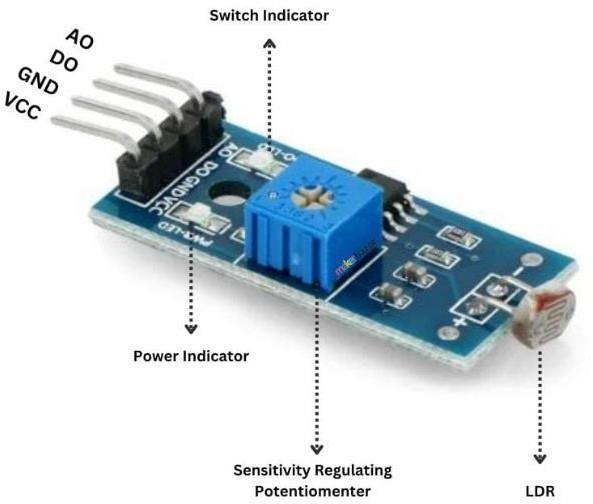
\includegraphics[width=48mm]{figures/fig8_ldr_sensor_module.jpg} &
    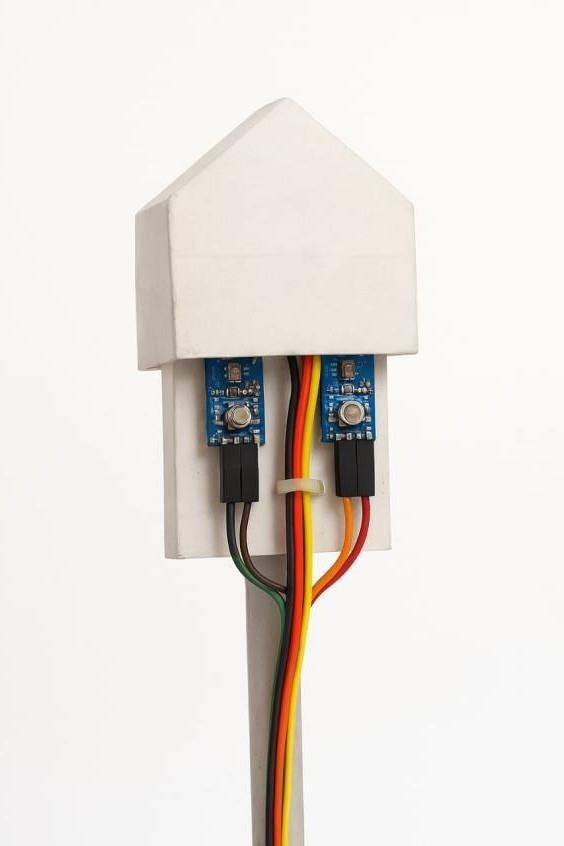
\includegraphics[width=42mm]{figures/fig8b_ldr_dual_module.jpg}
  \end{tabular}
\end{center}

\noindent
\begin{spacing}{1.2}
{\fontsize{10.2}{14.5}\selectfont
The LDR (Light Dependent Resistor) sensor module is used in this project to detect the intensity of sunlight and provide input to the Arduino Nano for automatic solar tracking. It works on the principle that the resistance of an LDR changes with the intensity of light falling on it.\\[3.5mm]
\textbf{Function:}
\begin{itemize}[leftmargin=8mm, itemsep=2mm, label=\textbullet]
  \item Two LDR modules are placed at slightly different positions on the parabolic collector.
  \item When sunlight intensity is unequal between the two sensors, the resistance difference creates a voltage difference.
  \item This voltage difference is sent to the Arduino Nano, which processes the signal.
  \item The Arduino then commands the motor driver to rotate the collector toward the side receiving less light, aligning it perfectly with the Sun.
  \item Once both LDRs sense equal sunlight, the system stops the motor --- indicating correct alignment.
\end{itemize}
}
\end{spacing}
\clearpage
